\chapter{Analyse von artverwandten Spielen zur Konzeptentwicklung}\label{sec:analysis}

Das grundlegende Spielkonzept von \say{Connecting-Minds} wird durch die Analyse verwandter Spiele, wie sie im Kapitel \emph{\nameref{sec:sota}} beschrieben sind, sowie durch weitere Spiele mit vergleichbarem Spieldesign ergänzt. Ziel ist es, durch diese vergleichende Betrachtung Gestaltungsprinzipien und Mechaniken zu identifizieren, die als Inspiration und konzeptionelle Grundlage für die Entwicklung von \say{Connecting-Minds} dienen können.

Darüber hinaus sollen die Ergebnisse dieser Analyse zur Beantwortung der zentralen Forschungsfrage, \emph{\say{Welche spezifischen Eigenschaften muss eine solche Umgebung aufweisen und welche Kommunikationsparameter werden dabei angesprochen?}}, beitragen.

\section{Methodik}
Zur systematischen Analyse der artverwandten Spiele wurde ein mehrstufiges, eigens entwickeltes Analyseraster herangezogen. Dieses Raster gliedert sich in vier aufeinander aufbauende Abschnitte:

\subsection{Visuelle Analyse}
Im ersten Schritt wurde der Fokus auf die sichtbaren Rätsel- und Hinweiselemente innerhalb des visuellen Designs der untersuchten Spiele gelegt. Relevante Elemente wurde direkt im Bildmaterial markiert, um sie im Rahmen der nachfolgenden Auswertung gezielt untersuchen zu können. Diese Markierungen dienten der Identifikation wiederkehrender Gestaltungselemente sowie der Kategorisierung der eingesetzt Rätseldesigns. Darüber hinaus konnten auf diese Weise Interaktionsflüsse sichtbar gemacht und chronologisch geordnet werden. Zusätzlich wurden die jeweiligen Kamera- und Perspektivführungen sowie Ansichten auf die Spielumgebung berücksichtigt, um Rückschlüsse auf das räumliche Design ziehen zu können.

\subsection{Erstellung eines Diagramms zur Rätselstruktur}
Anschließend wurden für ausgewählte Spielabschnitte oder komplette Spielverläufe UML-Ablaufdiagramme erstellt. Ziel war es, die strukturelle Organisation sowie die logische Verknüpfung und Verschachtelung der Rätselinhalte zu erfassen. Die Vorgehensweise orientiert sich an methodischen Ansätzen zur Rätselstrukturierung, wie sie bspw. von \cite{tim_schafer_grim_1996} vorgeschlagen wurden.

\subsection{Deskriptive Übertragung}
Im dritten Schritt erfolgt eine deskriptive Zusammenführung der aus der visuellen Analyse und der strukturellen Diagrammerstellung gewonnenen Erkenntnisse. Diese wurden hinsichtlich ihrer Implikationen für das Design und die Gestaltung von Rätseln systematisch beschrieben.

\subsection{Schlussfolgerung}
% Im letzten Schritt wurden die Beobachtungen aus den vorangegangenen Schritten in Bezug auf die Konzeptentwicklung von \say{Connecting-Minds} gesetzt und Rückschlüsse in das eigene Konzept eingearbeitet.
Abschließend wurden die zuvor gewonnen Beobachtungen in Beziehung zur Konzeptentwicklung von Connecting-Minds gesetzt. Dabei wurde untersucht, welche Elemente potenziell übernommen, angepasst oder vermieden werden sollten, Diese Rückschlüsse flossen gezielt in die Weiterentwicklung der eigenen Konzepts ein.

\section{Ergebnisse der Analysen}
In den einzelnen Kapiteln werden nun die Analysen zu den Spielen \say{We were here}, \say{We were here too}, \say{Tiny Room Stories} und \say{Myrmidon} vorgestellt.

\subsection{We were here - Spielreihe}
Es wurde sich hier nur auf die ersten zwei Teile (\say{We were here} und \say{We were here too}) der Spielreihe beschränkt, da der Umfang alle Spiele zu spielen und zu analysieren zu wenig Ertrag ergeben würde. Die Spiele wurden daher nur in der Breite  analysiert. Die beiden Spiele werden im Folgenden als ganzes betrachtet.

\paragraph{Visuelle Analyse}
Abbildungen \ref{} in Anhang [Anhang verlinken] und \ref{} in Anhang [Anhang verlinken] geben einen Einblick in die Analyse der Spieler-Rollen der Spiele. Schnell fällt auf, dass die Rätselelemente der Spiele sehr häufig über Symbole oder Bilder gestaltet wurden. Die Bilder oder Symbole müssen richtig ausgewählt und platziert werden.  Grundlegend sind Rätsel in der Spielwelt eingebaut. Das bedeutet, dass entweder Symbole an den Wänden zu sehen sind, oder Anweisungen in Textform in der Spielwelt integriert wurden. Selten ist es so, dass durch auditives Storytelling oder Texte in Büchern Rätsel gelöst werden müssen. In \say{We were here} fällt zudem auf, dass der \say{Explorer} die eingebauten Rätsel lösen muss während sich der \say{Librarian} in einer Hub befindet, über welchen er zu allen Rätseln die richtige Lösung finden muss. In \say{We were here too} ist es ähnlich. Häufig befindet sich der \say{Peasant} in Räumen mit den Rätseln und der \say{Lord} in den Räumen mit den Lösungen. Allerdings wurde hier öfters auch der \say{Lord} durch das Lösen von Rätseln gefordert. Außerdem befindet er sich nicht in einem zentralen Hub.

\paragraph{Analyse des Rätseldesigns}
Abbildung \ref{fig:wwh-uml} und \ref{fig:wwht-uml} im Anhang zeigen jeweils die Ablaufdiagramme von \say{We were here} und \say{We were here too}. Auffallend ist, dass in \say{We were here} die Rolle des \say{Librarian}s im Kontext des Rätseldesigns linear verläuft und nur selten verschachtelte Rätsel aufzufinden sind. Grundlegend ist es so, dass der \say{Explorer} auf die Rätsel und Hindernisse trifft, und der \say{Librarian} dafür zuständig ist, die richtigen Antworten zu liefern. Es findet eine sehr eindimensionale Verkettung zwischen den Rollen statt.
In \say{We were here too} lassen sich im Vergleich zum Vorgänger-Teil öfters verkettete Rätseldesigns finden. Zum Beispiel in Raum 2 des Spiels. Dies ist jedoch nur in Ausnahmen der Fall. Es wiederholt sich ein ähnlicher Aufbau wie im Vorgänger.
% \newpage
[kommt in Anhang, UML]

\begin{figure}[ht]
\centering
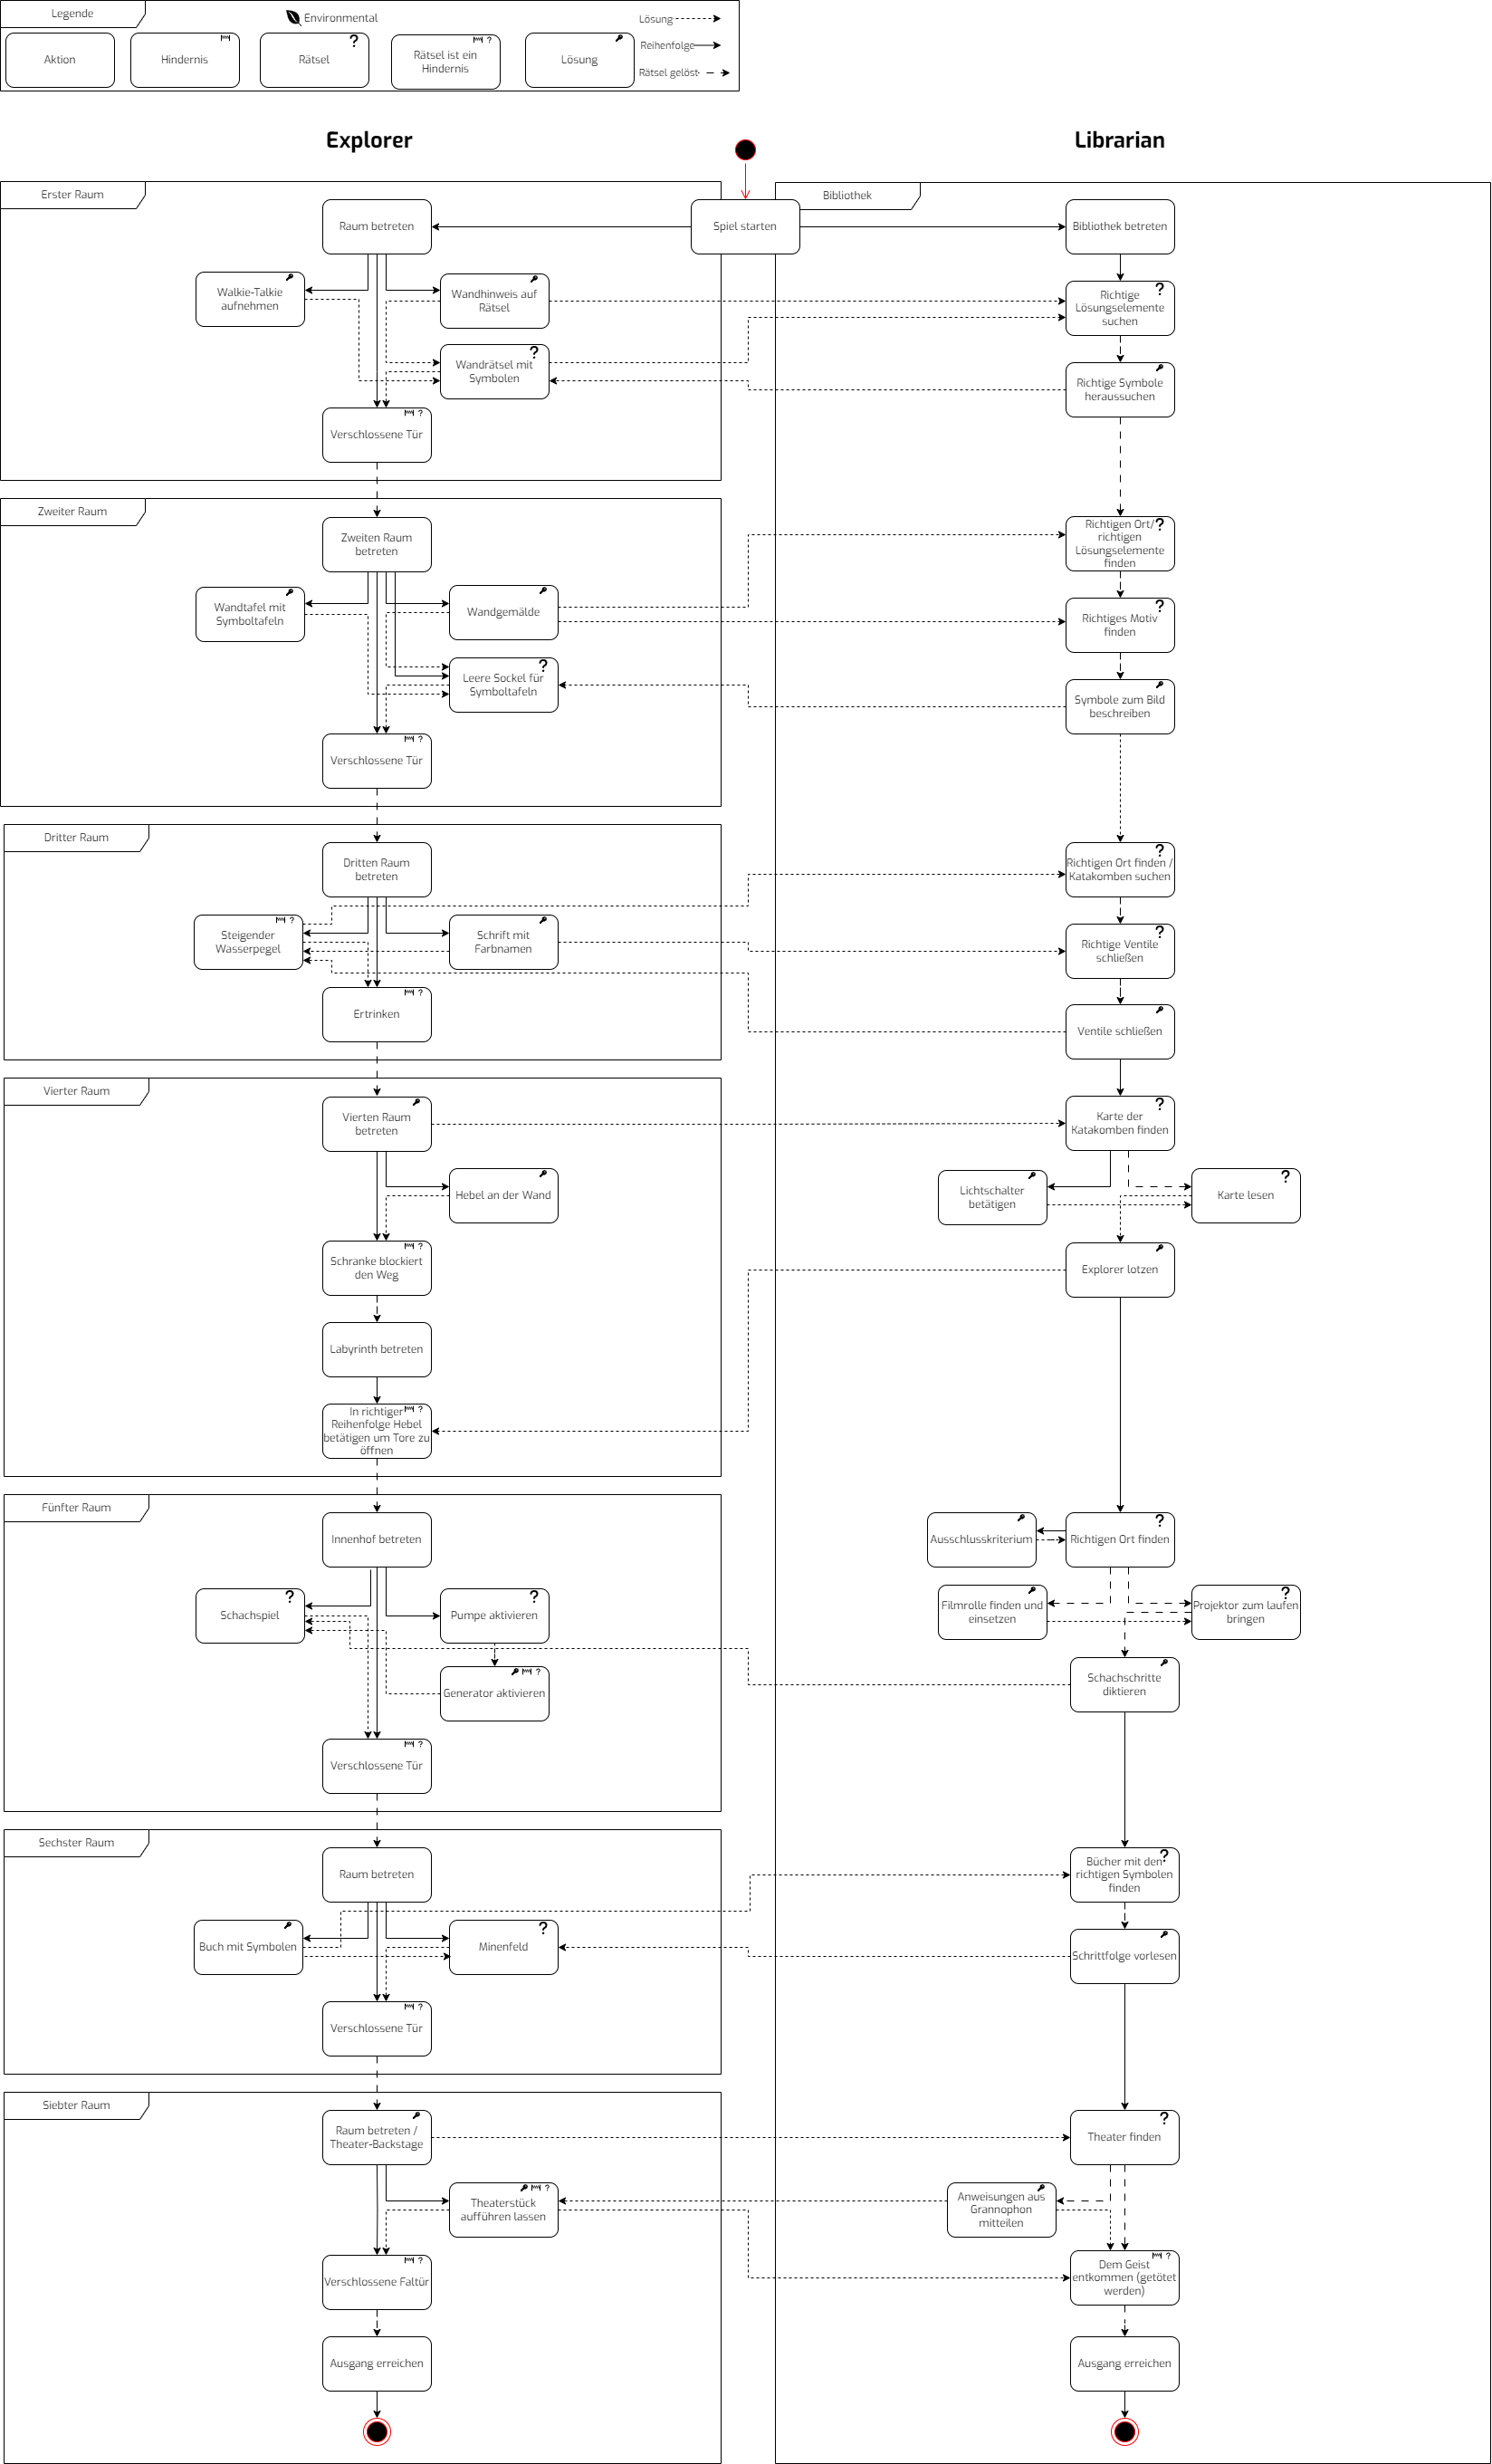
\includegraphics[width=0.8\linewidth]{content/pictures/WeWereHereUML.png}
\caption{Rätseldesign von We were here (Quelle: eigene Darstellung), vollständig in Anhang: }
\label{fig:wwh-uml}
\end{figure}

% \newpage
[kommt in Anhang, UML]
\begin{figure}[ht]
\centering
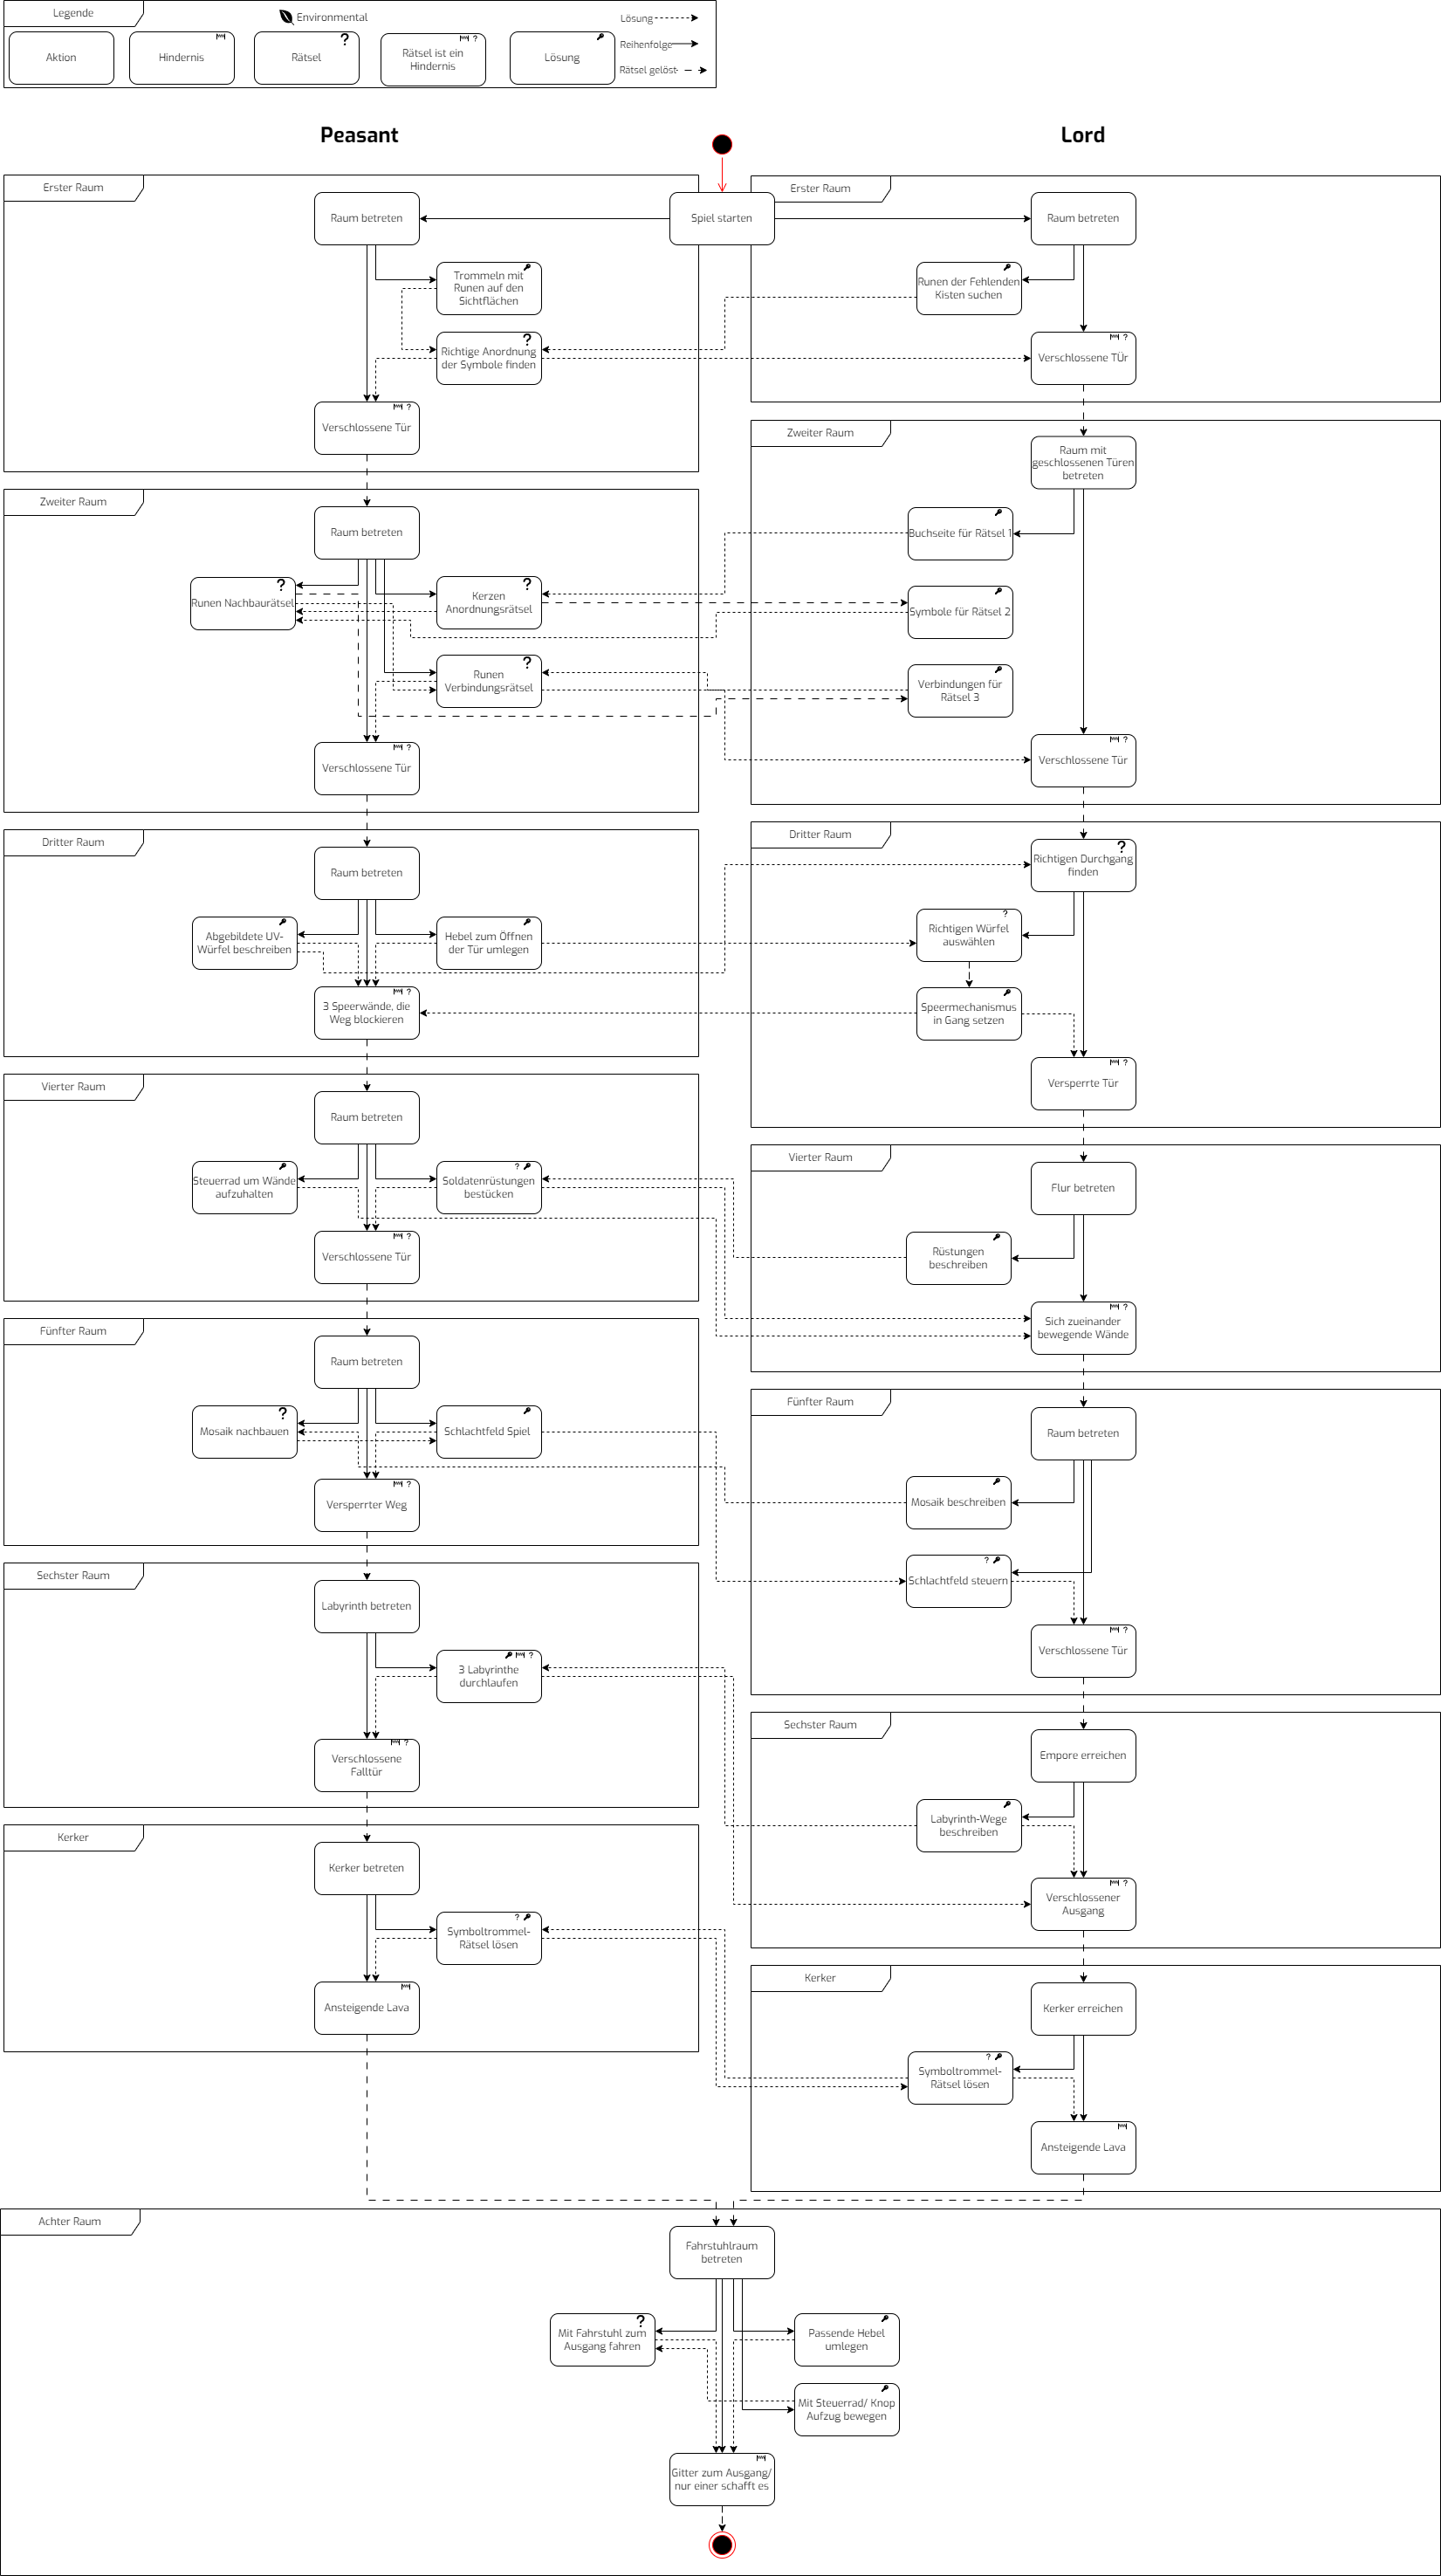
\includegraphics[width=0.8\linewidth]{content/pictures/WeWereHereTooUML.png}
\caption{Rätseldesign von We were here too (Quelle: eigene Darstellung), vollständig in Anhang: }
\label{fig:wwht-uml}
\end{figure}
% \newpage
% \newpage
\paragraph{Schlussfolgerung}
Der zentrale Aspekt der Kommunikationsaufforderung ist in beiden Spielen erkennbar. Er bildet eine gemeinsame Grundlage. In \say{We were here} fällt jedoch auf, dass das Rätseldesign häufig monoton und eindimensional wirkt - \say{Explorer} stößt auf Rätsel, beschreibt gegebene und/oder gesuchte Gegenstände, \say{Librarian} geht in bestimmten Raum und beschreibt gesuchte Gegenstände, \say{Explorer} löst Rätsel. Es existieren zwar einzelne Ausnahmen, in denen der \say{Librarian} aktiv werden muss um dem \say{Explorer} weiterzuhelfen - \say{Librarian} muss das richtige Ventil vom Rohr öffnen. Doch diese wechselseitige Abhängigkeit bleibt die Ausnahme. Gerade diese Form der Verzweigung ist für \say{Connecting-Minds} essenziell und sollte eine tragende Rolle Spielen. Auf dieser Grundidee lässt sich aufbauen, auch wenn nicht jedes Rätsel in seiner konkreten Ausgestaltung überzeugt, bieten bestimmte Ansätze dennoch wertvolle Anregungen - insbesondere im Hinblick auf die Möglichkeit, abwechslungsreiche, variantenreichere und stärker auf Kooperation ausgelegte Rätsel für \say{Connecting-Minds} zu entwickeln.

Deutlich weiter geht das zweite Spiel, \say{We were here too}, in dem die gegenseitige Verflechtung zwischen den beiden Rollen wesentlich häufiger zum Tragen kommt. In vielen Fällen ist es der \say{Peasant}, der nicht nur seinen eigenen Weg zum nächsten Raum freischaltet, sondern zugleich auch den vom \say{Lord}. In zwei Fällen ist das Prinzip sogar umgekehrt gestaltet: Der \say{Lord} ermöglicht dem \say{Peasant} den Zugang zu neuen Bereichen. In einem der beiden Fällen muss der \say{Peasant} eine Wendeltreppe hinaufrennen, unter der sich der Boden langsam einzieht. Er kommt jedoch nur bis zu einer Schwerwand, die über einen Würfel geöffnet werden kann. Er muss dem \say{Lord} den Aufschnitt des Würfels beschreiben, welcher den richtigen Würfel auswählen muss und in die Zielablage ablegen muss. Durch die Verschachtlung wird der Grundgedanke der Kommunikation und Zusammenarbeit deutlich verstärkt hervorgehoben und erzeugt ausgeglichenen Spaß in den Anwendungen. Ein weiterer Zusatz des Rätseldesigns ist das aufeinander Aufbauen von Rätseln. Dieses Element wird im Rahmen dieser Schlussfolgerung als \say{Mehrstufigkeit} bezeichnet und ist zum Beispiel in Raum 2 zu finden, bei dem aneinander gekettet, verschiedene Rätsel gelöst werden müssen.

Diese strukturelle Ausrichtung eignet sich grundsätzlich gut als gestalterische Vorlage, sofern sie sich sinnvoll in \say{Connecting-Minds} übertragen lässt. Gleichzeitig zielt \say{Connecting-Minds} auf eine noch tiefere und kontinuierliche Abhängigkeit zwischen den beiden Spielerrollen. Beide Rollen sollen nicht nur gelegentlich, sondern regelmäßig und systematisch aufeinander angewiesen sein - die Zusammenarbeit wird damit zur unverzichtbaren Grundlage des Spielfortschritts. Aus der engen Verflechtung ergibt sich, dass Kooperation nicht nur hilfreich, sondern spielentscheidend wird.

Konzepte wie mehrstufige Rätsel oder Einsatz von zeitlichen Begrenzungen (Timer) sind in diesem Zusammenhang ebenfalls interessante Überlegungen. Während Mehrstufigkeit sich als zentrales Element für die Rätselgestaltung anbietet, sollte der Timer gezielt und situationsabhängig eingesetzt werden, da sein Einfluss stark vom jeweiligen Spannungsbogen und dem beabsichtigten Spielerlebnis abhängt.

\subsection{Tiny Room Stories}
Im Vergleich zur \say{We were here}-Reihe ist Tiny Room Stories ein Singelplayer-Spiel bei dem alleine Rätsel gelöst werden müssen. die Abschnitte und Informationen für die Geschichte des Spiels freischalten. Betrachtet wurden in der Analyse der Prolog und Kapitel 1 des Spiels. Der Aufbau der weiteren Kapiteln ist identisch und verändert sich nur im Inhalt des Designs und der Verschachtlung der Rätsel und Hinweise.

\paragraph{Visuelle Analyse}
Die Abbildungen \ref{} und \ref{} in den Anhängen [Anhang verlinken] und [Anhang verlinken] zeigen die Ergebnisse dieser ersten Analyse. Der Fokus liegt zunächst auf den Informationen und Anweisungen die der Spieler vom Spiel erhält. Sie wird fortgesetzt mit der Identifizierung der Rätselarten und wie diese gelöst werden. Außerdem wurde ein Fokus auf die Steuerungshinweise gelegt, um zu bestimmen, welche Steuerungselemente in die Konzeptentwicklung von \say{Connecting-Minds} übernommen werden können. Im allgemeinen besitzt das Spiel \say{Tiny Room Stories} in das Environment eingebettete Rätsel und Hinweise auf die Rätsel. Diese werden ergänzt durch Hinweisnotizen, die das narrative Rätseldesign darstellen. Die zwei Designansätze unterstützen sich gegenseitig und bieten abwechslungsreiche und teilweise herausfordernde Rätsel.

\paragraph{Analyse des Rätseldesigns}
Abbildung \ref{fig:trs-uml} zeigt das Ablaufdiagramm der Rätsel des Spiels. Sowohl in der visuellen Darstellung des Spiels, als auch im Design der Rätsel ist erkennbar, dass Zugänge zu neuen Räumen neue Hinweise oder Rätsel freischalten, welche gelöst werden müssen. Die Rätsel sind dabei gegenseitig verwoben, sodass es oft vorkommt, dass das Lösen von Rätsel A erst Hinweise für Rätsel B zugänglich macht wodurch Rätsel C ebenso gelöst werden kann. Diese Struktur findet sich in Kapitel 1 beim Bücherregal Rätsel wieder, als auch bereits im Prolog beim Öffnen der Schranke.

\begin{figure}[ht]
\centering
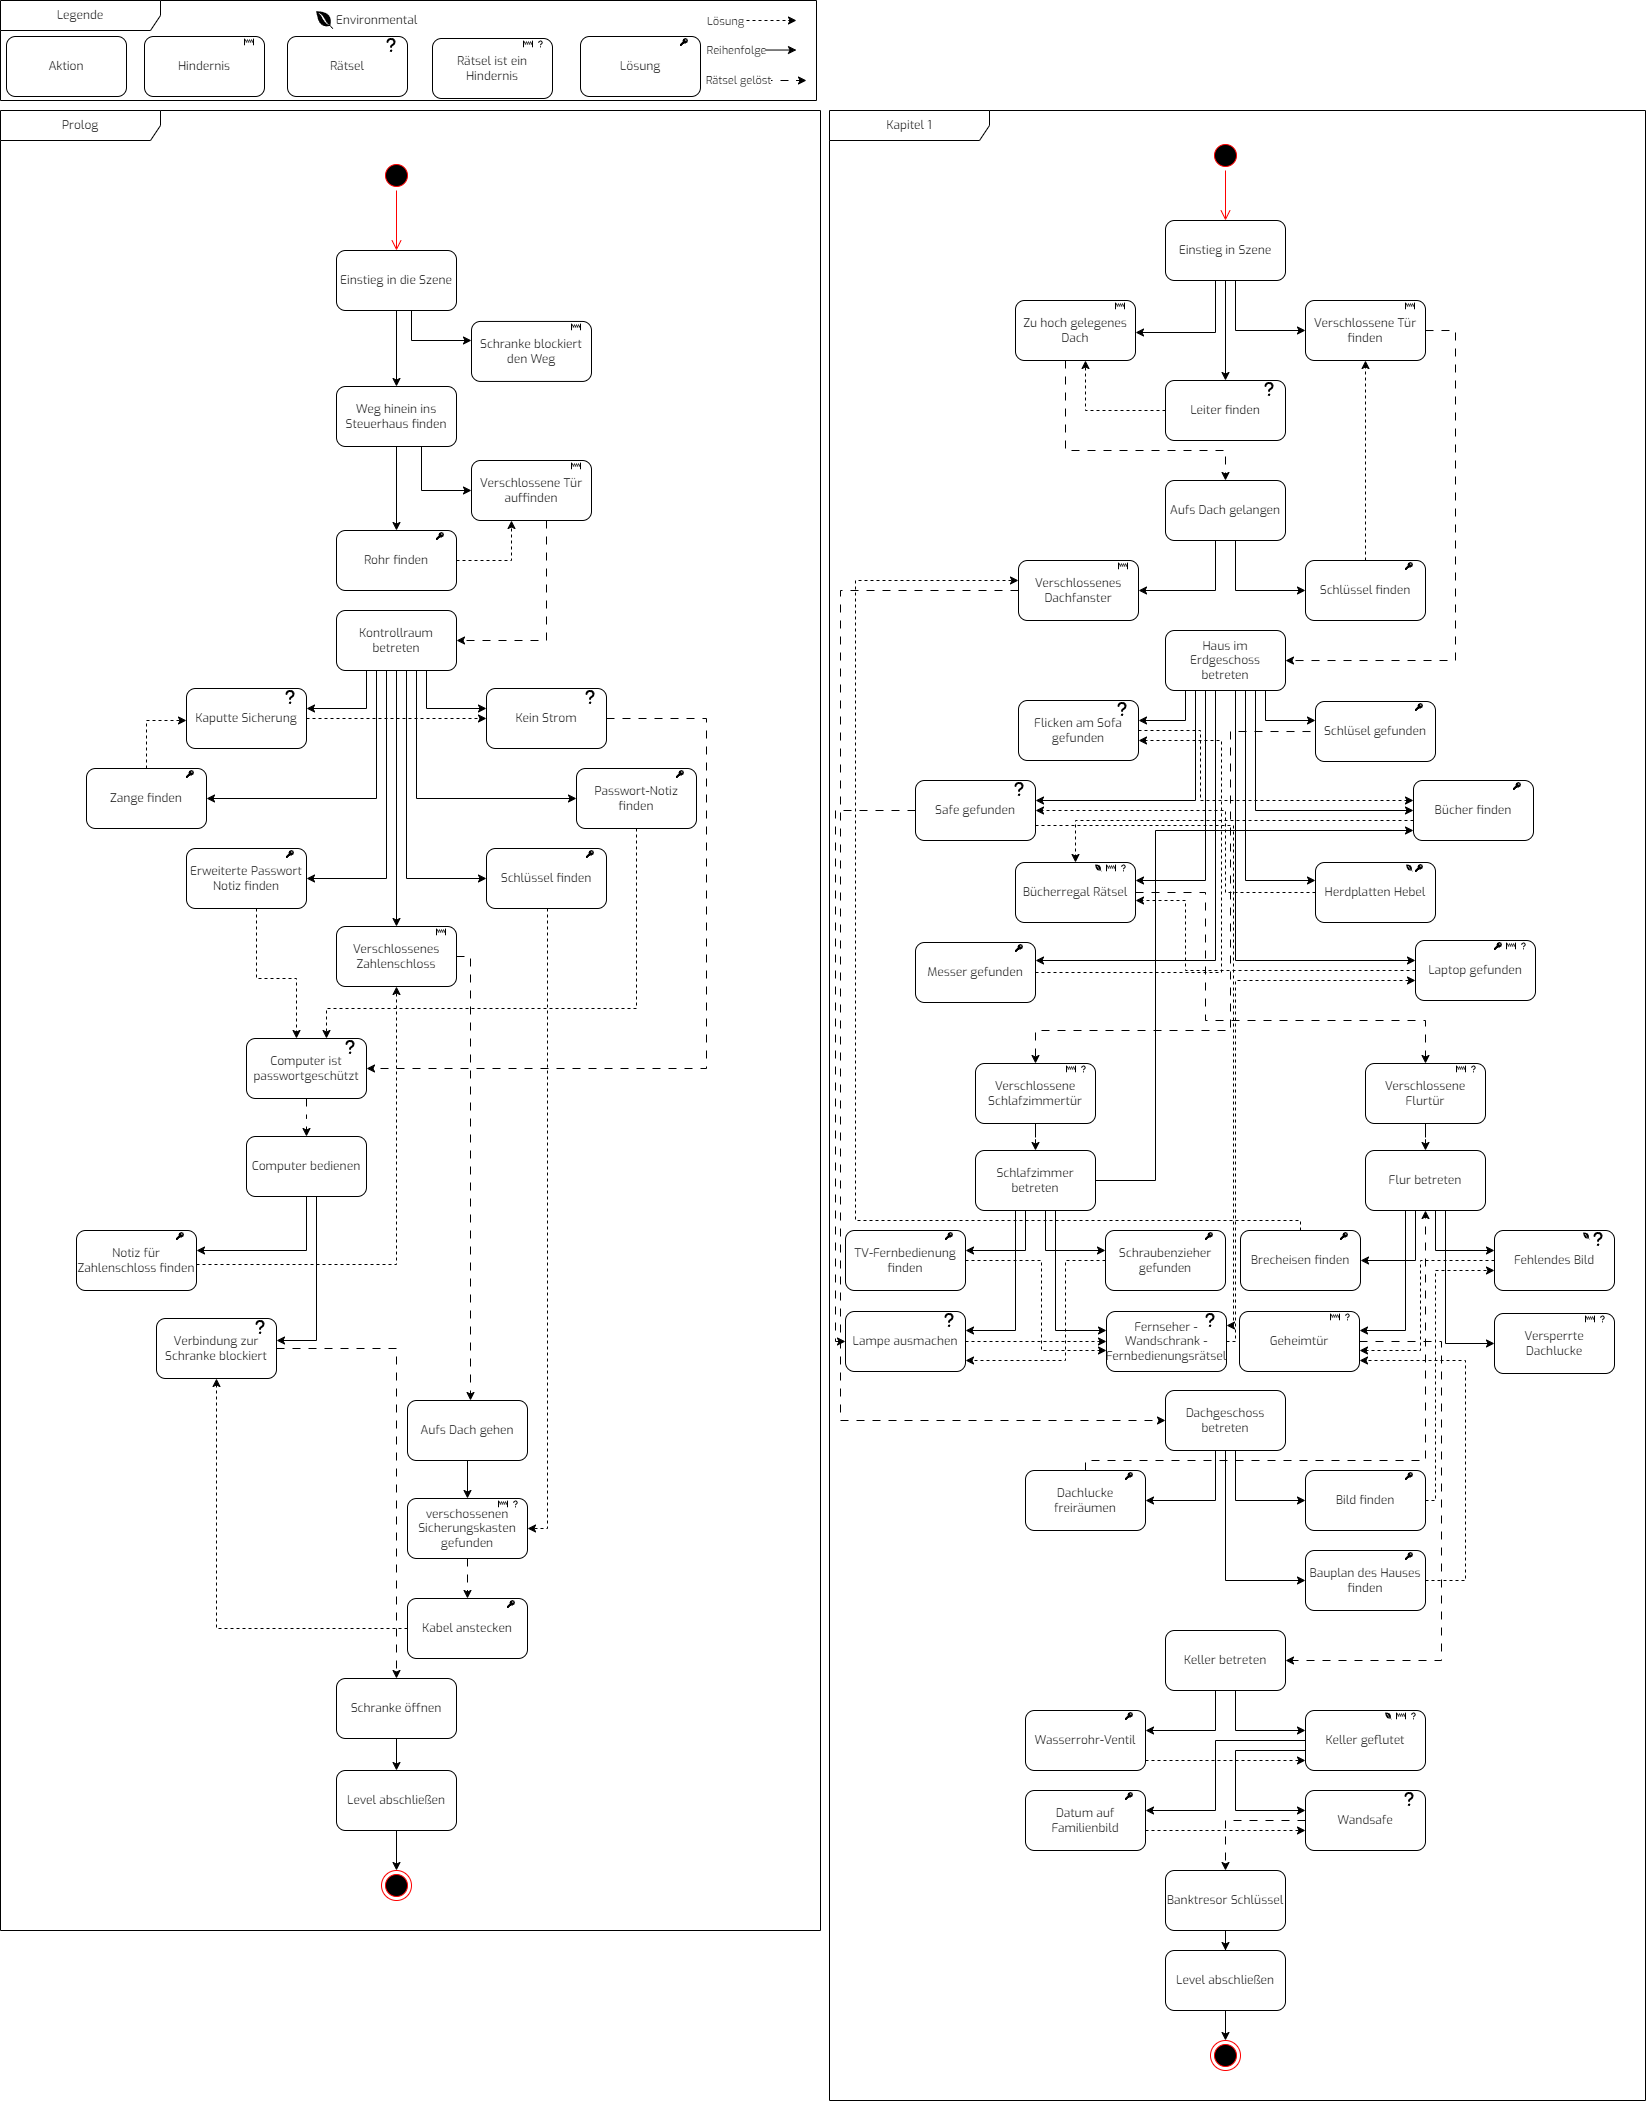
\includegraphics[width=1\linewidth]{content/pictures/TinyRoomStoriesUML.png}
\caption{Rätseldesign von Tiny Room Stories (Quelle: eigene Darstellung), vollständig in Anhang: }
\label{fig:trs-uml}
\end{figure}

\paragraph{Schlussfolgerung}
Die Spielsteuerung kann eine gute Vorlage für \say{Connecting-Minds} bietet. Zum einen überzeugt sie durch ihre klare und intuitive Umsetzung, die gut auf diesen Prototyp übertragbar sein kann. Zum anderen passt die Struktur der Rätsel ausgezeichnet zu der Art und Weise, wie die Aufgaben der zwei Spielerrollen gestaltet sein könnten.

Besonders interessant ist dabei, wie sich untergeordnete und übergeordnete Rätsel sinnvoll miteinander verknüpfen lassen. Die Rolle des einen Spielers löst oder entdeckt ein Element, dessen Erkenntnis der andere Spieler anschließend aktiv umsetzen muss, um wiederum des einen Spielers die nächsten Schritte ermöglicht. Dieses Prinzip des wechselseitigen Fortschritt eröffnet spannende Möglichkeiten für das Rätseldesign von \say{Connecting-Minds}.

\subsection{Myrmidon}
Das Spiel \say{Myrmidon} reiht sich in die Spiele der asymmetrischen Multiplayer wie die \say{We Were Here}-Reihe ein. Es müssen kooperativ Wege freigelegt und ermöglicht werden. Die Analyse des Spiels umfasst das anfängliche Tutorial. Es unterscheidet sich lediglich in der szenischen Einbettung der Spielerrolle der animierten Puppe. Im Tutorial ist die Ausgestaltung der Welt identisch zu der, die der Animator sieht. Im Hauptteil des Spiel, das nur aus dem Tutorial und einem ersten richtigen Level besteht, wird die Szenerie der Puppe in einen Stop-Motion-Film eingebettet. Der Animator hingegen sieht eine interaktive Kulisse, mit wenig Dekoration.

\paragraph{Visuelle Analyse}
Die Abbildungen \ref{} und \ref{} in den Anhängen [Anhang bennen] zeigen die Ergebnisse der ersten Analyse. Nach dem Zusammenfinden in einer Lobby wählen die Spieler ihre jeweilige Rolle innerhalb einer kooperativen Dyade aus. Die Rollenverteilung ist dabei asymmetrisch. Eine Person übernimmt die Rolle des \say{Animators}, die andere die der \say{Stop-Motion Puppe}. Die visuelle Gestaltung orientieren sich dabei stark an einem stilisierten Stop-Motion-Film. 
Der \say{Animator} steuert dabei die Kamera in einem offenen, dreidimensionalen Raum und ist für die aktive Gestaltung der Kulisse verantwortlich. Diese Kulisse bildet den Bewegungsraum für die \say{Puppe}, deren Fortschritt vom Eingreifen des Animators abhängt. So muss der Animator im Tutorial durch das Öffnen von Schubladen eine provisorische Treppe errichten, damit die Puppe die höhergelegene Kisten und Schrankfächer erreichen kann. 
Manche der benötigten Elemente befinden sich zunächst nicht im Zugriff des Animators, sondern sind in verschiebbaren Kisten in der Spielwelt enthalten. Erst wenn diese Kisten durch die Puppe aus der Spielwelt hinausgeschoben wurden,  werden die enthaltenen Kulissenteile im Spielraum des Animators interagierbar. Dieser kann sie anschließend an vorbestimmten Bereichen, z. B. einer Korkwand, Haltestangen oder Falltüren platzieren, um der Puppe neue Wege zu ermöglichen.
Die Puppe hingegen wird in der Spielwelt eines Stop-Motion-Films bewegt. Sie sieht den Außenbereich, den der Animator sieht, nicht. Aufgrund limitierter Kameraansichten ist die Puppe an manchen Stellen auf die verbale Navigation des Animators angewiesen. Die Kommunikation zwischen beiden Rollen ist somit essenziell, da viele Hindernisse nur durch gemeinsames Planen und Koordinieren überwindbar sind.

\paragraph{Analyse des Rätseldesigns}
Abbildung \ref{fig:myrmidon-uml} zeigt das Rätseldesign des Tutorials. Auffallend ist, dass beide Spieler dem Weg der Puppe folgen müssen um an das Ziel des Abschnitts zu gelangen. Auf diesem Weg gerät die Puppe an Hindernisse, die der Animator durch das Interagieren mit der Spielkulisse beseitigen kann. Nachdem beide Spieler die Spielwelt betreten haben, muss der Animator seiner Puppe einzelne Schubladen in einem kleinen Schreibtischschränkchen öffnen, damit die Puppe die Schubladen als eine Art Leiter nutzen kann. Weitere Arten von \say{Rätsel} bzw. Hindernisse, die beseitigt werden müssen, sind mehrstufig verbunden. Das bedeutet, der Animator muss zwar der Puppe eine Bewegungsmöglichkeit in die Kulisse bauen, allerdings muss die Puppe dafür zunächst diese Bewegungsmöglichkeit freischalten. Dies geschieht in der Mitte des Tutorials, bei dem die Puppe zunächst eine Kiste aus der Spielwelt schieben muss, damit die enthaltene Stange an die Wand gesteckt werden kann, damit die Puppe über die Stange über einen Abgrund springen kann.
Das letzte Hindernis im Tutorial besteht aus der Kombination aus Schubladen in der Kulisse öffnen und Hilfsmöglichkeiten durch die Puppe freischalten. Im weiteren Verlauf des Spiels wiederholen sich diese 3 Arten von Rätsel. 
\begin{figure}[ht]
\centering
\includegraphics[width=0.8\linewidth]{content/pictures/RätseldesignMyrmidon.png}
\caption{Rätseldesign des Tutorials von Myrmidon (Quelle: eigene Darstellung)}
\label{fig:myrmidon-uml}
\end{figure}

\paragraph{Schlussfolgerung}
Aus der Visuellen Analyse und der Analyse des Rätseldesigns geht hervor, dass einige Parallelen zur Spielidee von Connecting-Minds existieren. Die größte Parallele existiert im Freischalten und Nutzen von Gegenständen um gemeinsam Hindernisse zu überwinden. Die größten Unterschiede bestehen allerdings in der Darstellung des anderen Spieleravatars in der eigenen Anwendung. Im Connecting-Minds soll der Watcher den Avatar des Players in der Spielwelt nicht sehen. Es soll die Kommunikation durch das Beschreiben der derzeitigen Position gefördert werden. Außerdem ist die Hauptaufgabe des Animators auf das Unterstützen der Puppe beschränkt. Es existieren keine Abschnitte, in denen der Animator für sich Umgebungsrätsel oder Hindernisse lösen muss. Dieser Aspekt soll in Connecting-Minds für den Watcher umgesetzt werden. An diesen Abschnitten muss dann sogar der Player dem Watcher unterstützen. 

\section{Zusammenfassung und Interpretation der Ergebnisse}
Die Analyse der vier Vergleichsspiele zeigt, dass das Zusammenspiel zwischen asymmetrischen Rollen, sowie die Gestaltung konzentrationsfördernden Rätseln  bereits in einigen Spielen enthalten sind, allerdings auch gute Vorlagen bieten können um neue Ideen zu entwickeln.
Die größte Relevanz für das Konzept von Connecting-Minds ergibt sich aus der engen wechselseitigen Abhängigkeiten der Spielerrollen, wie sie insbesondere in \say{We Were Here Too} sowie \say{Myrmidon} erkennbar sind.

Während \say{We Were Here} nur punktuell auf gegenseitige Interaktion setzt und häufig ein eher eindimensionales Rätselmuster verfolgt, gelingt es dem Nachfolger \say{We Were Here}, die strukturelle Defizite aufzugreifen und durch eine stärkere verzahnte Aufgabenverteilung zu ergänzen. Die wechselseitigen Bedingtheit von Fortschritt erzeugt nicht nur eine höhere kommunikative Dichte, sondern verankert Kooperation als auch spielentscheidendes Element. Konzepte wie Mehrstufigkeit und temporale Elemente (z. B. Timer) erscheinen in diesem Kontext als potenzielle Designprinzipien für Connecting-Minds, deren gezielter Einsatz sowohl die Spannung als auch das Bedürfnis nach synchronisierter Zusammenarbeit steigern kann.

Auch \say{Tiny Room Stories} liefert wertvolle Impulse für Connecting-Minds, insbesondere durch seine klar strukturierte Steuerung, sowie die Verknüpfung aus über- und untergeordneter Rätselkomponenten. Die Idee, dass eine Spielhandlung des einen Spielers zu einer neuen Möglichkeit für den anderen führt, unterstützt die Vision von einem dynamischen, bidirektionalen Spielfluss. Das Prinzip des \say{wechselseitigen Fortschritts} lässt sich als zentrales Designziel ableiten.

Die Analyse von \say{Myrmidon} zeigt, dass bestimmte Parallelen zu Connecting-Minds bereits bestehen. Darunter zählt das wechselseitige Freischalten und Nutzen von Gegenständen zur Überwindung gemeinsamer Hindernisse. Zugleich treten zentrale Unterschiede hervor, etwa in der Sichtbarkeit des anderen Spielers in der Spielwelt. Während in \say{Myrmidon} die Puppe in der Kulisse des Animators visuell präsent ist, wird in Connecting-Minds gezielt darauf gesetzt, dass die Position des Players nur der Player kennt. Dadurch soll die verbale Kommunikation und räumliche Beschreibung gefördert werden.
Darüber hinaus offenbart \say{Myrmidon} eine einseitige Aufgabenverteilung. Der Animator dient als Unterstützer für seine Stop-Motion-Puppe. Das lösen von eigenständigen oder durch die Puppe unterstützende Rätsel oder Hindernisse wurden nicht realisiert. Diese Arbeit hingegen zielt genau darauf ab, dass der Watcher an gewählten Abschnitten Rätsel lösen muss. Unterstützt wird er dafür vom Player. Dies soll eine stärker balancierte Kooperationsstruktur ermöglichen. Dieser wechselseitiger Rollenwechsel ist in den analysierten Vergleichsspielen bislang kaum ausgeprägt und stellt damit ein potenzielles Alleinstellungsmerkmal von Connecting-Minds dar.

\section{Methodendiskussion}\label{sec:analysis-discussion}
Diese Kapitel umfasst die kritische Auseinandersetzung des gewählten methodischen Vorgehens.

Zunächst wurde für diese Arbeit kein standardisiertes Vorgehen zur Analyse der Spiele angewandt. Die Arbeit wurde aufgrund des Wunsches nach zielgerichteter Informationssammlung durchgeführt. Ein standardisiertes Vorgehen, wie dem \ac{MDA}-Framework (vgl. \cite{hunicke_mda_2004}) oder anhand der \ac{CMP} (vgl. \cite{seif_el-nasr_understanding_2010}), hätte vermutlich zu einem ähnlichen Ergebnis führen können, wäre in seiner Durchführung jedoch umfangreicher gewesen.
Außerdem stellt diese Art der Analyse eine ausschließlich subjektive Meinung des Erstellers dar.

Ein Aspekt der in der Analyse der Spiele fehlt ist die statistische Bestimmung von Schwierigkeitsgraden, bspw. die der enthaltenen Rätsel. Hierbei wurde keine Metrik gefunden, anhand welcher bestimmt werden kann, wie einfach oder schwer manche Abschnitte sind. Entweder weil sie ein komplexes Pattern-Rekognition voraussetzen oder einfach nur bestimmte Elemente gespeichert werden müssen. Eine solche Metrik kann auch bei der Konzeption und Entwicklung eigener Rätsel vor Vorteil sein, um etwa abschätzen zu können, bei welchen Rätseln mehrere Lösungshinweise eingebaut werden müssen.

Außerdem wurden auch gezielt einige Spiele aus Kapitel \ref{sec:sota} ausgeschlossen, da diese entweder in ihrer Art zu verschieden sind (It Takes Two) oder der Kooperative Teil viel zu überraschend auftritt (The past within). Die Spiele It Takes Two und Split Fiction wurden ausgeschlossen, da sie zwar in weiten Teilen ein asymmetrisches Kooperatives Spiel sind, jedoch die Avatare der einzelnen Spielerrollen in der gleichen Spielwelt umher gehen, sich gegenseitig sehen und interagieren können. Keep Talking and Nobody Explodes bildet den grundlegenden Gedanken eines asymmetrischen kooperativen Spiels bei verschiedenen Aufgabengebieten vollumfänglich ab, jedoch sind die Aufgabengebiete zu sehr geteilt, sodass keine bidirektionale Ereignisse ausgelöst werden. Eine gewünschte Bidirektionalität des Spiels ist hier nicht gegeben. The past within wurde ebenfalls aus der Analyse ausgeschlossen, da zwischen einigen Rätseln, die selbständig in der jeweiligen Anwendung der Dyade gelöst werden müssen, das kooperative Rätsel lösen implementiert wurde. Das lösen der Rätsel findet lediglich durch vorlesen der Lösungen statt.  Auch in seiner Art der Rätsel unterschiedet sich das Design des Spiels von der Idee von Connecting-Minds und konnte daher weniger dazu beitragen, das eigene Konzept weiterzuentwickeln.

